%----------------------------------------------------------------------------------------
%	PACKAGES AND OTHER DOCUMENT CONFIGURATIONS
%----------------------------------------------------------------------------------------

\documentclass[
11pt, % The default document font size, options: 10pt, 11pt, 12pt
%oneside, % Two side (alternating margins) for binding by default, uncomment to switch to one side
english, % ngerman for German
singlespacing, % Single line spacing, alternatives: onehalfspacing or doublespacing
%draft, % Uncomment to enable draft mode (no pictures, no links, overfull hboxes indicated)
%nolistspacing, % If the document is onehalfspacing or doublespacing, uncomment this to set spacing in lists to single
%liststotoc, % Uncomment to add the list of figures/tables/etc to the table of contents
%toctotoc, % Uncomment to add the main table of contents to the table of contents
%parskip, % Uncomment to add space between paragraphs
%nohyperref, % Uncomment to not load the hyperref package
headsepline, % Uncomment to get a line under the header
%chapterinoneline, % Uncomment to place the chapter title next to the number on one line
%consistentlayout, % Uncomment to change the layout of the declaration, abstract and acknowledgements pages to match the default layout
]{style} % The class file specifying the document structure

\usepackage[utf8]{inputenc} % Required for inputting international characters
\usepackage[T1]{fontenc} % Output font encoding for international characters

\usepackage{mathpazo} % Use the Palatino font by default

\usepackage[backend=bibtex,style=authoryear,natbib=true]{biblatex} % Use the bibtex backend with the authoryear citation style (which resembles APA)

\addbibresource{./misc/bibliography.bib} % The filename of the bibliography

\usepackage[autostyle=true]{csquotes} % Required to generate language-dependent quotes in the bibliography

\usepackage{hyperref}% http://ctan.org/pkg/hyperref

%----------------------------------------------------------------------------------------
%	MARGIN SETTINGS
%----------------------------------------------------------------------------------------

\geometry{
	paper=a4paper, % Change to letterpaper for US letter
	inner=2.5cm, % Inner margin
	outer=3.8cm, % Outer margin
	bindingoffset=.5cm, % Binding offset
	top=1.5cm, % Top margin
	bottom=1.5cm, % Bottom margin
	%showframe, % Uncomment to show how the type block is set on the page
}

%----------------------------------------------------------------------------------------
%	THESIS INFORMATION
%----------------------------------------------------------------------------------------

\thesistitle{Automated Malware Analysis Using Large Language Models} % Your thesis title, this is used in the title and abstract, print it elsewhere with \ttitle
\supervisor{Dr Robert G \textsc{Smith}} % Your supervisor's name, this is used in the title page, print it elsewhere with \supname
\examiner{} % Your examiner's name, this is not currently used anywhere in the template, print it elsewhere with \examname
\degree{M.Sc} % Your degree name, this is used in the title page and abstract, print it elsewhere with \degreename
\author{Andre M M \textsc{Faria}} % Your name, this is used in the title page and abstract, print it elsewhere with \authorname
\addresses{Dublin, Ireland} % Your address, this is not currently used anywhere in the template, print it elsewhere with \addressname

\subject{Applied Cybersecurity} % Your subject area, this is not currently used anywhere in the template, print it elsewhere with \subjectname
\keywords{} % Keywords for your thesis, this is not currently used anywhere in the template, print it elsewhere with \keywordnames
\university{\href{https://www.tudublin.ie/}{Technological University Dublin}} % Your university's name and URL, this is used in the title page and abstract, print it elsewhere with \univname
\department{\href{https://www.tudublin.ie/explore/faculties-and-schools/computing-digital-data/informatics-and-cybersecurity/}{School of Informatics and Cyber Security}} % Your department's name and URL, this is used in the title page and abstract, print it elsewhere with \deptname
\submitdate{May 2025} % The month and year that you submit your FINAL draft to the university, this is not currently used anywhere in the template, print it elsewhere with \subdate

\AtBeginDocument{
\hypersetup{pdftitle=\ttitle} % Set the PDF's title to your title
\hypersetup{pdfauthor=\authorname} % Set the PDF's author to your name
\hypersetup{pdfkeywords=\keywordnames} % Set the PDF's keywords to your keywords
}

\begin{document}

\frontmatter % Use roman page numbering style (i, ii, iii, iv...) for the pre-content pages

\pagestyle{plain} % Default to the plain heading style until the thesis style is called for the body content

%----------------------------------------------------------------------------------------
%	TITLE PAGE
%----------------------------------------------------------------------------------------

\begin{titlepage}
	\begin{center}

		\vspace*{.06\textheight}
		{\scshape\LARGE \univname\par}\vspace{1.5cm} % University name
		\textsc{\Large Masters Thesis}\\[0.5cm] % Thesis type

		\HRule \\[0.4cm] % Horizontal line
		{\huge \bfseries \ttitle\par}\vspace{0.4cm} % Thesis title
		\HRule \\[1.5cm] % Horizontal line

		\begin{minipage}[t]{0.4\textwidth}
			\begin{flushleft} \large
				\emph{Author:}\\
				\href{https://www.linkedin.com/in/andremmfaria/}{\authorname} % Author name - remove the \href bracket to remove the link
			\end{flushleft}
		\end{minipage}
		\begin{minipage}[t]{0.4\textwidth}
			\begin{flushright} \large
				\emph{Supervisor:} \\
				\href{https://www.tudublin.ie/explore/faculties-and-schools/computing-digital-data/informatics-and-cybersecurity/people/academic-staff/robertsmith.php}{\supname} % Supervisor name - remove the \href bracket to remove the link
			\end{flushright}
		\end{minipage}\\[2cm]

		\vfill

		\large \textit{A thesis submitted in fulfillment of the requirements\\ for the degree of \degreename\\ in \subjectname}\\[0.4cm] % University requirement text
		\textit{in the}\\[0.4cm]
		\deptname\\[2cm] % Research group name and department name

		
\includegraphics[width=0.2\textwidth]{./images/uni-logo.png} % University/department logo - uncomment to place it

		\vfill

		{\large \subdate}\\[4cm] % Date

		\vfill
	\end{center}
\end{titlepage}

%----------------------------------------------------------------------------------------
%	DECLARATION PAGE
%----------------------------------------------------------------------------------------

\begin{declaration}
	\addchaptertocentry{\authorshipname} % Add the declaration to the table of contents
	\noindent I, \authorname, declare that this thesis titled, \enquote{\ttitle} and the work presented in it are my own. I confirm that:

	\begin{itemize}
		\item This work was done wholly or mainly while in candidature for a research degree
		      at this Institute of Technology Blanchardstown.
		\item Where any part of this thesis has previously been submitted for a degree or any
		      other qualification at this University or any other institution, this has been
		      clearly stated.
		\item Where I have consulted the published work of others, this is always clearly
		      attributed.
		\item Where I have quoted from the work of others, the source is always given. With
		      the exception of such quotations, this thesis is entirely my own work.
		\item I have acknowledged all main sources of help.
		\item Where the thesis is based on work done by myself jointly with others, I have
		      made clear exactly what was done by others and what I have contributed
		      myself.\\
	\end{itemize}

	\noindent Signed:\\
	\rule[0.5em]{25em}{0.5pt} % This prints a line for the signature

	\noindent Date: \today \\
	\rule[0.5em]{25em}{0.5pt} % This prints a line to write the date
\end{declaration}

\cleardoublepage

%----------------------------------------------------------------------------------------
%	QUOTATION PAGE
%----------------------------------------------------------------------------------------

\vspace*{0.2\textheight}

\noindent\enquote{\itshape The true thesis are the friends we make along the way.}\bigbreak

\hfill Anonymous

%----------------------------------------------------------------------------------------
%	ABSTRACT PAGE
%----------------------------------------------------------------------------------------

\begin{abstract}
	\addchaptertocentry{\abstractname} % Add the abstract to the table of contents
	Despite the fact that an abstract is quite brief, it must do almost as much
	work as the multi-page paper that follows it. In a computer science paper, this
	means that it should in most cases include the following sections. Each section
	is typically a single sentence, although there is room for creativity. In
	particular, the parts may be merged or spread among a set of sentences. Use the
	following as a checklist for your next abstract (URL:
	http://www.ece.cmu.edu/~koopman/essays/abstract.html):

	\begin{description}
	\item[Motivation:] Why do we care about the problem and the results? If the problem
			isn't obviously "interesting" it might be better to put motivation first; but
			if your work is incremental progress on a problem that is widely recognized as
			important, then it is probably better to put the problem statement first to
			indicate which piece of the larger problem you are breaking off to work on.
			This section should include the importance of your work, the difficulty of the
			area, and the impact it might have if successful.
	\item[Problem statement:] What problem are you trying to solve? What is the scope of
			your work (a generalized approach, or for a specific situation)? Be careful not
			to use too much jargon. In some cases it is appropriate to put the problem
			statement before the motivation, but usually this only works if most readers
			already understand why the problem is important.
	\item[Approach:] How did you go about solving or making progress on the problem? Did
			you use simulation, analytic models, prototype construction, or analysis of
			field data for an actual product? What was the extent of your work (did you
			look at one application program or a hundred programs in twenty different
			programming languages?) What important variables did you control, ignore, or
			measure?
	\item[Results:] What's the answer? Specifically, most good computer architecture
			papers conclude that something is so many percent faster, cheaper, smaller, or
			otherwise better than something else. Put the result there, in numbers. Avoid
			vague, hand-waving results such as "very", "small", or "significant." If you
			must be vague, you are only given license to do so when you can talk about
			orders-of-magnitude improvement. There is a tension here in that you should not
			provide numbers that can be easily misinterpreted, but on the other hand you
			don't have room for all the caveats.
	\item[Conclusions:] What are the implications of your answer? Is it going to change
			the world (unlikely), be a significant "win", be a nice hack, or simply serve
			as a road sign indicating that this path is a waste of time (all of the
			previous results are useful). Are your results general, potentially
			generalizable, or specific to a particular case?

	\end{description}
\end{abstract}

%----------------------------------------------------------------------------------------
%	ACKNOWLEDGEMENTS
%----------------------------------------------------------------------------------------

\begin{acknowledgements}
	\addchaptertocentry{\acknowledgementname} % Add the acknowledgements to the table of contents
	The acknowledgments and the people to thank go here, don't forget to include your project advisor\ldots
\end{acknowledgements}

%----------------------------------------------------------------------------------------
%	LIST OF CONTENTS/FIGURES/TABLES PAGES
%----------------------------------------------------------------------------------------

\tableofcontents % Prints the main table of contents

\listoffigures % Prints the list of figures

\listoftables % Prints the list of tables

%----------------------------------------------------------------------------------------
%	ABBREVIATIONS
%----------------------------------------------------------------------------------------

\begin{abbreviations}{ll} % Include a list of abbreviations (a table of two columns)

	\textbf{LAH} & \textbf{L}ist \textbf{A}bbreviations \textbf{H}ere\\
	\textbf{WSF} & \textbf{W}hat (it) \textbf{S}tands \textbf{F}or\\

\end{abbreviations}

%----------------------------------------------------------------------------------------
%	PHYSICAL CONSTANTS/OTHER DEFINITIONS
%----------------------------------------------------------------------------------------

\begin{constants}{lr@{${}={}$}l} % The list of physical constants is a three column table

	% The \SI{}{} command is provided by the siunitx package, see its documentation for instructions on how to use it

	Speed of Light & $c_{0}$ & \SI{2.99792458e8}{\meter\per\second} (exact)\\
	%Constant Name & $Symbol$ & $Constant Value$ with units\\

\end{constants}

%----------------------------------------------------------------------------------------
%	SYMBOLS
%----------------------------------------------------------------------------------------

\begin{symbols}{lll} % Include a list of Symbols (a three column table)

	$a$ & distance & \si{\meter} \\
	$P$ & power & \si{\watt} (\si{\joule\per\second}) \\
	%Symbol & Name & Unit \\

	\addlinespace % Gap to separate the Roman symbols from the Greek

	$\omega$ & angular frequency & \si{\radian} \\

\end{symbols}

%----------------------------------------------------------------------------------------
%	DEDICATION
%----------------------------------------------------------------------------------------

\dedicatory{For/Dedicated to/To my\ldots}

%----------------------------------------------------------------------------------------
%	THESIS CONTENT - CHAPTERS
%----------------------------------------------------------------------------------------

\mainmatter % Begin numeric (1,2,3...) page numbering

\pagestyle{thesis} % Return the page headers back to the "thesis" style

% Include the chapters of the thesis as separate files from the Chapters folder
% Uncomment the lines as you write the chapters

%----------------------------------------------------------------------------------------

% Define some commands to keep the formatting separated from the content 
\newcommand{\keyword}[1]{\textbf{#1}}
\newcommand{\tabhead}[1]{\textbf{#1}}
\newcommand{\code}[1]{\texttt{#1}}
\newcommand{\file}[1]{\texttt{\bfseries#1}}
\newcommand{\option}[1]{\texttt{\itshape#1}}

%----------------------------------------------------------------------------------------

% Chapter 1

\chapter{Introduction}
\label{sec:introduction}

\label{Chapter1} % For referencing the chapter elsewhere, use \ref{Chapter1} 

Ever since the creation of the first computer by Charles Babbage in the 19th century, computers
have been evolving at a rapid pace performing more and more tasks as the time passes. With this
evolution, malicious actors began to notice manners in which to subvert established systems. These
individuals, by force of belief or personal gain, have caused losses in the trillions to
organizations and individuals across the globe.

As a response to these threats, these organizations and individuals began to develop techniques and
tools to counter malicious actors. It has then, started the cat-and-mouse race between criminals
and agents of the law. One of these techniques revolves around the analysis of what software
adversaries develop to understand how they operate and the vulnerabilities they exploit to weaken
or outright topple established security systems.

This thesis presents a research about, and creation of, a method where RAG powered LLMs are
introduced onto to the malware static analysis workflow in order to increase efficiency on the
analysis.

\section{Definitions}
Here are defined all of the concepts and/or tools that are mentioned.

\subsection{Large Language Models}
Large Language Models (LLMs) are a type of multi-parameter Machine Learning (ML) algorithm designed
for natural language processing. These models that are trained on a large volume of text using a
multitude of learning techniques such as supervised and self-supervised learning.

Generative pre-trained transformers (GPTs) are the biggest and most powerful LLMs. Current models
can be adapted to certain tasks (via fine-tuning) or directed by prompt engineering
	[\cite{brown2020languagemodelsfewshotlearners}]. These models learn to predict the syntax,
semantics and ontologies found in human language, but they also pick up biases and errors from the
training data [\cite{10.1162/daed_a_01905}]. Popular examples of LLMs include:
\begin{itemize}
	\item GPT models (like GPT-4 or ChatGPT)
	\item Google's PaLM and Gemini
	\item Meta Llama series models
\end{itemize}

\subsection{Retrieval-Augmented Generation}
Retrieval-Augmented Generation (RAG) is a technique that allows for LLMs to query information from
a specific type of datastore and use it as context for the response it provides. This allows for
adaptive learning of the models without the need of retraining (fine-tuning). It improves the
quality of LLM output as the model does not rely solely on pre-trained knowledge but also on
relevant information from the datastore.

RAG works by having the LLM to query the datastore using vector search, embeddings or keyword
matching (depending on the datastore type), feeding this data onto the LLM input and then
continuing with the normal LLM process for output generation.

\subsection{Malware}
Short for \textit{Malicious Software}, Malware is any program or code that is created for malicious
purposes like exploitation of computer systems networks or users. Often created with monetary gain
in mind, these programs activities include stealing sensitive data, damage systems, disrupt
operations or gain unauthorized access to systems or environments. Common types of malware include:
\begin{itemize}
	\item Viruses: Attach themselves to legitimate software, spreading when the software is run.
	\item Worms: Spread automatically over networks, replicating rapidly without user intervention.
	\item Trojans: Disguised as legitimate software, tricking users into installing them to enable
	      unauthorized access.
	\item Ransomware: Encrypts or locks files, demanding payment (ransom) for restoration.
	\item Spyware: Secretly collects sensitive information like passwords or browsing activity.
	\item Adware: Delivers unwanted advertisements, potentially slowing down or compromising systems.
\end{itemize}

\subsection{Malware Analysis}
As mentioned before, the software created by malicious actors needs to be evaluated and analyzed to
understand how it works, what exploits it takes advantage of and how these exploits can be patched.
As a basis, there are two types of analysis of software that can be made to understand any kind of
software. These are as follows:
\begin{itemize}
	\item \textbf{Static Analysis}: Focuses on looking at the sequences of individual instructions on the software
	      bytecode to identify the its characteristics, such as identification of the parameters in which the
	      analyzed software is built upon (e.g. Operating system it executes on, processor architecture,
	      etc), what execution paths it employs, what system calls it performs, etc. This analysis is done
	      without running the code and it requires a lot of time and effort from the analyst.
	\item \textbf{Dynamic Analysis}: Entails running the potential malicious software to gather runtime information such as network calls
	      and system call execution data which are not visible through static analysis. This analysis is done by creating a special (sandbox) environment (i.e docker container and/or a virtual machine) and running the software.
\end{itemize}

\subsubsection{Static vs Dynamic Analysis}

% \vfill
% 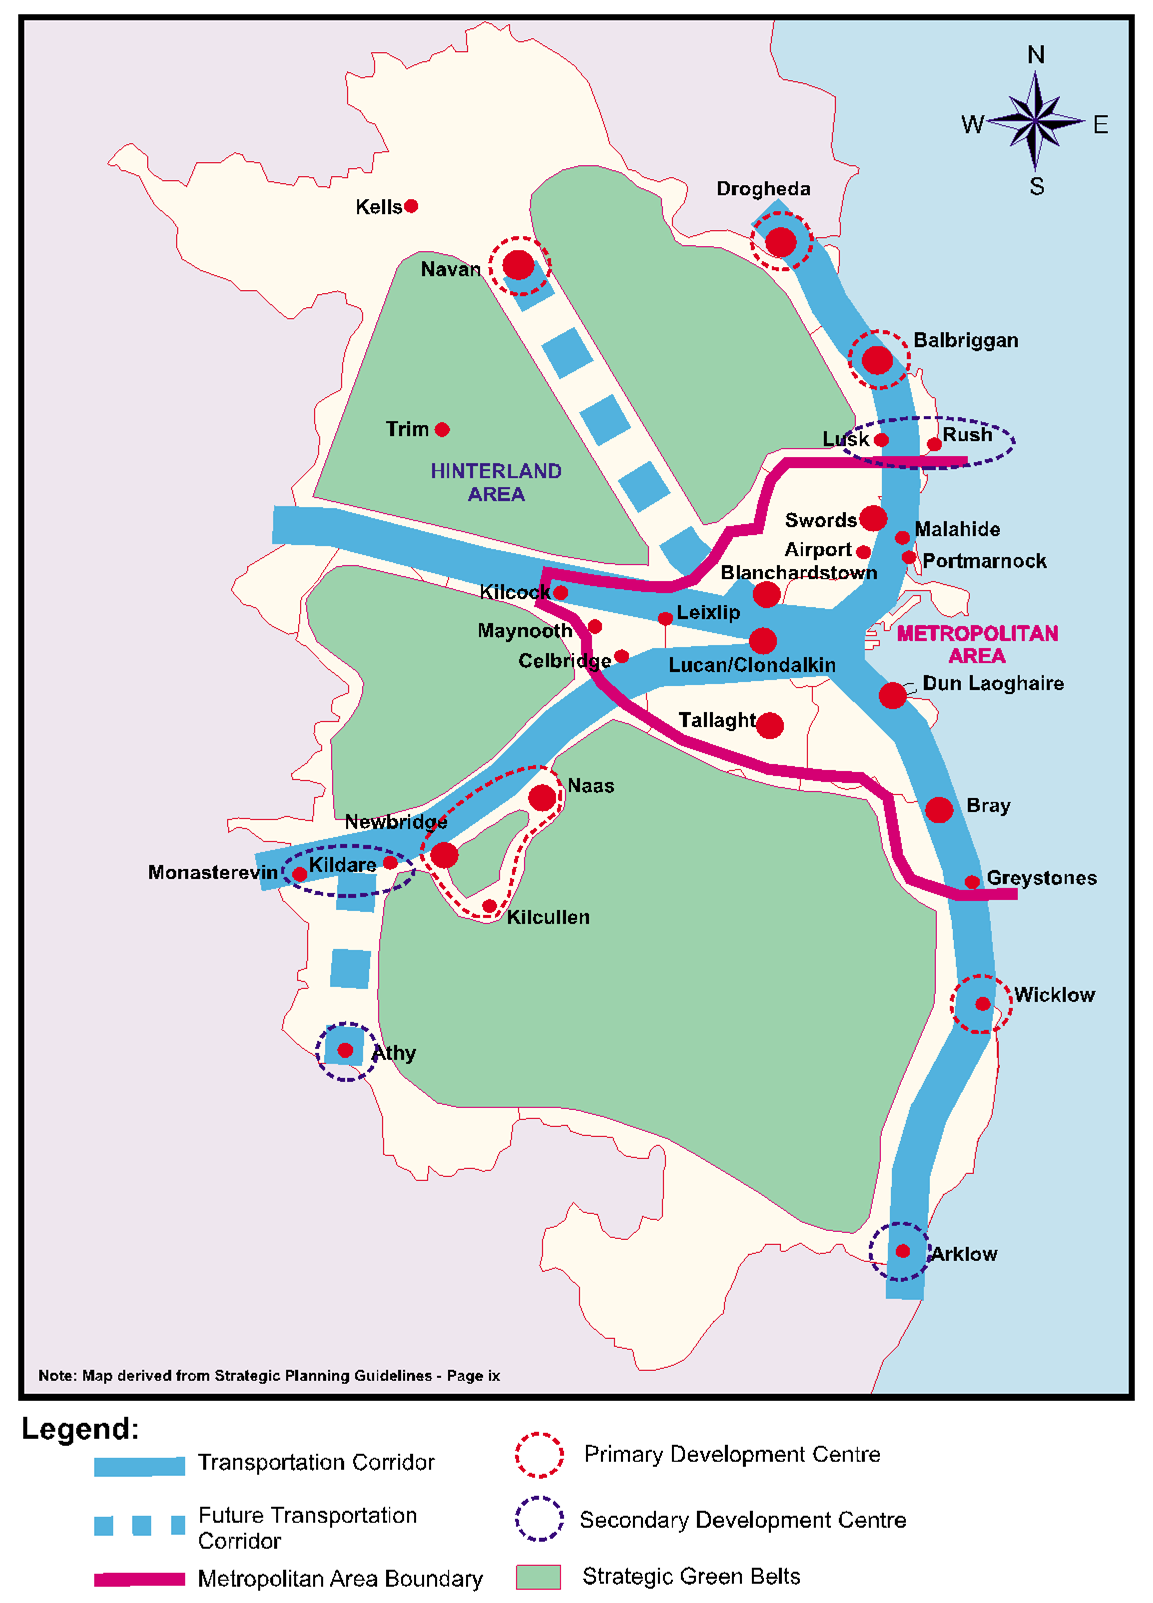
\includegraphics[width=\textwidth]{intro1.png}
% \vfill

\section{Research questions and objectives}

\subsection{Questions}
These are the research questions that will guide the development of this thesis.
\begin{itemize}
	\item How LLMs can be leveraged to enhance static malware analysis?
	\item How does a RAG-enhanced LLM compare to traditional static analysis techniques in terms of accuracy,
	      efficiency, and interpretability?
	\item What role does RAG play in improving LLM-driven malware classification, particularly in terms of
	      contextual relevance and justifiability of results?
\end{itemize}

\subsection{Objectives}
\begin{itemize}
	\item Develop a method for integrating LLMs with RAG to enhance static malware analysis.
	\item Evaluate the effectiveness of RAG-enhanced LLMs in identifying, explaining, and comparing malware
	      threats using static features (e.g., file structure, bytecode, API calls) against traditional
	      static malware analysis techniques in terms of accuracy, efficiency, and interpretability, while
	      identifying challenges and potential risks (e.g., adversarial manipulation and hallucination).
\end{itemize}

% \section{Section Introduction}
% %always begin a section with an introduction and end it with a summery
% A thesis is built up of a series of chapters that construct a substantiated and convincing response
% to the research question(s). Typically, a thesis contains the following chapters: an introduction;
% a literature review; a description of methodology; a report and discussion of results; and a
% conclusion. A thesis may have five to eight chapters depending on the nature of the study, the
% required word count and the requirements of the degree.

% \subsection{About the Introduction Chapter}
% An introduction is crucial to setting the tone of your thesis – it is the first impression you’ll
% make on your readers (assessors). Briefly, it presents the purpose, context and scope of your
% research. Likewise, a conclusion is just as crucial – it is the lasting impression you’ll make on
% your readers (assessors). Not only does it give a summary of your thesis, but should provide a
% clear, convincing answer to your research question(s).
% \subsection{Subsection header 2}
% After introducing your work, you should list your research questions, hypothesis, and objectives.

% Always keep in mind the meaning of the word ``\textit{Thesis}''. That is: a thesis is a statement
% or theory that is put forward as a premise to be maintained or proved. A Hypo\textit{thesis} then,
% is a sub-thesis, or a smaller part of the overarching thesis.

% All of your research questions must aim to prove or disprove your thesis.. and thus your
% hypotheses.

% See more here: \url{https://www.statconsul.com/research-questions.php}
% \subsection{Subsection header 3}
% The last thing you do in an Introduction Chapter is to outline the contents of your thesis, i.e., a
% review of then literature is provided in Chapter \ref{sec:LitReview}, starting with... etc...
% Chapter \ref{sec:Method} provides a description of the method... etc...

% \section{More about the Introduction chapter}
% The introduction allows you to orient the reader to your research project and preview the
% organisation of your thesis. In the introduction, state what the topic is about, explain why it
% needs to be further researched and introduce your research question(s) or hypothesis.

% Whilst patterns of organisation in introductions vary, there are some common features that will
% help you to achieve an informative and engaging introduction. Let’s identify these features:

% \begin{itemize}
% 	\item Introduce the topic
% 	\item Define key terms and concepts
% 	\item Give background and context for the topic (this may include a brief literature review)
% 	\item Review and evaluate the current state of knowledge in the topic (this may include a brief
% 	      literature review)
% 	\item Identify any gaps, shortcomings and problems in the research to date
% 	\item Introduce your research question(s) or hypothesis
% 	\item Briefly describe your methodology and/or theoretical approach
% 	\item Explain the aim of your research and what contribution it will make to the topic
% 	\item Give an overview of the chapter outline of the thesis.
% \end{itemize}

% It’s important to note that, depending on your field of study and the faculty requirements of your
% thesis, not all of these features will be relevant. Also, these features may occur in varied
% orders.

% Most people write many drafts of their introduction. It can be useful to write one early in the
% research process to clarify your thinking. You will need to write a version for your confirmation
% proposal and other milestones. As your research progresses and your ideas develop, you will need to
% revise it. When the final draft of chapters is complete, check the introduction once more to make
% sure that it accurately reflects what you have actually done.

\chapter{Literature Review}
\label{sec:LiteratureReview}
\label{Chapter2} % For referencing the chapter elsewhere, use \ref{Chapter2} 

% Briefly introduce the purpose of this chapter.
% Mention the key themes: static malware analysis, LLMs in cybersecurity, and RAG.
% Explain that the chapter identifies trends, evaluates contributions, and
% exposes gaps to justify your research.
TODO...

\section{Static Malware Analysis}
% Define static malware analysis and explain its significance.
% Discuss techniques such as:
%   - Signature-based detection
%   - Heuristic or rule-based analysis
%   - ML-based static classifiers
%     Highlight the limitations: poor generalization, obfuscation resistance,
%     lack of semantic context.
TODO...

\subsection{Signature-Based and Heuristic Methods}
% Describe traditional approaches and tools (e.g., YARA, ClamAV, AV engines).
% Mention why they’re fast but limited by pattern-dependence.
TODO...

\subsection{Machine Learning-Based Approaches}
% Explore the use of static features (e.g., API calls, bytecode) in ML models.
% Reference key datasets and benchmarks (e.g., EMBER, VirusShare).
% Highlight common issues: feature engineering overhead, poor explainability.
TODO...

\section{The Role of Language Models in Cybersecurity}
% Introduce LLMs (e.g., GPT, BERT, CodeBERT) in the context of cybersecurity.
% Highlight their ability to reason over code, extract threats, or assist in SOC workflows.
% Note both advantages (generalization, language reasoning) and challenges
% (hallucinations, black-box nature).
TODO...

\section{Retrieval-Augmented Generation (RAG) in NLP}
% Explain what RAG is: a combination of retrieval models and LLMs.
% Describe how it improves factuality and context-awareness in LLM outputs.
% Mention successful applications in NLP (e.g., QA, summarization).
% Start hinting at its potential benefits for malware analysis tasks.
TODO...

\section{Combining RAG and LLMs for Static Malware Analysis}
% Present any research, even conceptual, that combines RAG with malware classification.
% If the field is sparse, note how work in adjacent fields (e.g., RAG + code understanding) inspires your direction.
% Discuss why this integration can help with:
%   - Context-aware detection/classification
%   - Explainability of decisions
%   - Reducing hallucination by grounding in known malware samples/docs
TODO...

\section{Gaps in Current Literature}
% Identify clear gaps and connect them to your research questions.
% Examples:
%   - Few works integrate RAG with static analysis for malware
%   - LLM evaluations often ignore interpretability
%   - No benchmarking of RAG-LLM models vs traditional static tools
% Use this section to justify your proposed method and scope.
TODO...

\section{Summary}
% Recap key points and themes from the chapter.
% Mention how insights from the literature guide your upcoming methodology.
% Emphasize how your work addresses the identified gaps and pushes the field
% forward.
TODO...
 
\chapter{Methodology}
\label{sec:Method}
\label{Chapter3} % For referencing the chapter elsewhere, use \ref{Chapter3}

% Introduce the purpose of this chapter.
% Reiterate your research aim: enhancing static malware analysis with LLMs and RAG.
% Provide a brief overview of the methodology, including data sources,
% architecture, evaluation strategy, and toolchain.
TODO...

\section{Research Design}
% Describe the nature of your research: exploratory, experimental, comparative.
% Explain the reasoning for using a prototype-based implementation and evaluation.
% Emphasize that your approach avoids LLM fine-tuning and instead relies on
% prompt engineering and external context via RAG.
TODO...

\section{System Architecture}
% Provide a high-level description of your system pipeline.
% Include a diagram (later) showing flow: malware sample → static feature extraction → retrieval → prompt generation → LLM response.
% List major system components and their interactions.
TODO...

\section{Data Sources}
% Describe where you obtain your malware samples and intelligence documents.
% Malware sources:
%   - MalwareBazaar for static binaries and metadata.
%   - VirusTotal (optional, via API) for reports and behavior data.
%     Detail any preprocessing steps: parsing PE headers, extracting bytecode,
%     API call strings, etc.
TODO...

\section{Retrieval-Augmented Generation (RAG) Pipeline}
% Explain how RAG is constructed using Haystack and pgvector.
% Describe:
%   - Embedding model used to vectorize documents.
%   - How documents (e.g., malware reports) are stored in PostgreSQL.
%   - How semantic retrieval is performed and injected into the LLM prompt.
%     Clarify how this improves contextual relevance and grounding in known
%     threat data.
TODO...

\section{Prompt Engineering}
% Discuss how you craft prompts for different tasks: classification, explanation, and comparison.
% Include examples of how static features and retrieved context are structured in the prompt.
% Explain the decision to use GPT-4 and/or DeepSeek-R1 in inference-only mode.
TODO...

\section{Toolchain}
This section outlines the used tooling for the experiments and some discussion
on why they were chosen.

\subsection{Programming Language and Environment}
% Python is used for implementation.
% PDM (Python Development Master) manages dependencies and virtual environments.
TODO...

\subsection{Language Models}
% GPT-4 (via OpenAI API) and/or DeepSeek-R1 are used for inference.
% Models are not fine-tuned; they rely on prompt engineering and external
% retrieval for task performance.
TODO...

\subsection{RAG Framework and Storage}
% Haystack is used to build the retrieval pipeline.
% PostgreSQL with pgvector is used to store and query vector embeddings of
% malware-related documents.
TODO...

\subsection{Malware Intelligence Sources}
% MalwareBazaar is used to obtain real-world malware samples and metadata.
% VirusTotal may be used (via API) to enrich data with threat reports and
% behavioral indicators.
TODO...

\subsection{Evaluation and Visualization}
% Scikit-learn is used to compute performance metrics (e.g., accuracy, F1 score).
% Pandas and Matplotlib are used for data handling and visualization.
% All experiments are version-controlled and reproducible via PDM.
TODO...

\section{Evaluation Framework}
% Define your evaluation metrics: accuracy, efficiency, interpretability.
% Describe baseline comparisons against traditional static malware classifiers (if applicable).
% Discuss any human-in-the-loop components for evaluating explanation quality.
TODO...

\section{Reliability, Validity, and Limitations}
% Discuss how reproducibility is ensured via version control, fixed seeds, and public datasets.
% Address limitations:
%   - Limited to static analysis.
%   - Dependent on retrieval quality and LLM reliability.
%   - No user-study or adversarial robustness testing (unless planned).
TODO...

\section{Ethical Considerations}
% Ensure ethical use of malware datasets.
% Describe safety protocols: no execution of live malware, all samples are statically analyzed.
% Highlight responsible use of LLMs and privacy-conscious data handling if using
% VirusTotal.
TODO...

\section{Summary}
% Recap the methodology structure and justify how it addresses your research questions.
% Set up the transition into the next chapter, where implementation details or
% results will follow.
TODO...

\chapter{Discussion of Results}
\label{sec:Results}
\label{Chapter4} % For referencing the chapter elsewhere, use \ref{Chapter4} 

% Briefly restate the research objectives and the purpose of this chapter.
% Provide an overview of the key findings from your study.
% Outline how the discussion is structured to interpret these findings.
TODO...

\section{Summary of Key Findings}
% Concisely summarize the main results obtained from your experiments or analyses.
% Highlight findings related to the integration of LLMs and RAG in static malware analysis.
% Avoid detailed data presentation; focus on overarching outcomes.
TODO...

\section{Interpretation of Findings}
% Interpret the significance of your results in the context of your research questions.
% Discuss how the integration of LLMs and RAG has impacted malware detection accuracy, efficiency, and interpretability.
% Compare your findings with existing literature, noting agreements or discrepancies.
% Explain any unexpected results and explore possible reasons for these
% outcomes.
TODO...

\section{Implications of the Study}
% Discuss the practical implications of your findings for cybersecurity practices.
% Consider how your research can influence future malware analysis methodologies.
% Reflect on the potential for integrating LLMs and RAG in other areas of
% cybersecurity.
TODO...

\section{Limitations}
% Acknowledge the limitations of your study, such as dataset constraints, model biases, or scope restrictions.
% Discuss how these limitations may have influenced your results and interpretations.
% Provide a balanced view to demonstrate critical engagement with your research.
TODO...

\section{Recommendations for Future Research}
% Suggest areas where further investigation is warranted based on your findings.
% Propose how future studies can address the limitations identified.
% Consider recommending the exploration of dynamic analysis integration or
% real-world deployment evaluations.
TODO...

\section{Conclusion}
% Summarize the key points discussed in this chapter.
% Reinforce how your findings contribute to the field of static malware analysis.
% Provide a closing reflection on the overall significance of your research.
TODO...
 
% Chapter 5

\chapter{Conclusion}
\label{sec:Conclusion}

\label{Chapter5} % For referencing the chapter elsewhere, use \ref{Chapter5} 

\section{About Conclusions}
Depending on the type of research presented in the thesis, conclusion chapters
or sections tend to include at least some of the following:

\begin{itemize}
	\item A clear answer to your research question or hypothesis
	\item Summary of the main findings or argument
	\item Connections between your findings or argument to other research
	\item Explanation and significance of the findings
	\item Implications of the findings
	\item Limitations of the research and methodology
	\item Recommendations for future research
\end{itemize}

Your conclusion chapter is the place to emphasise the new knowledge that you’ve
contributed to the field of study and explain its significance. This chapter is
your opportunity to leave a strong impression on the reader (assessors) about
the strength and relevance of your research, and your skills as a researcher.

Importantly, the conclusion chapter must link with your introduction chapter to
complete the framing of the thesis and demonstrate that you have achieved what
you set out to do.
 

%----------------------------------------------------------------------------------------
%	THESIS CONTENT - APPENDICES
%----------------------------------------------------------------------------------------

\appendix % Cue to tell LaTeX that the following "chapters" are Appendices

% Include the appendices of the thesis as separate files from the Appendices folder
% Uncomment the lines as you write the Appendices

\appendix

\chapter{Frequently Asked Questions} % Main appendix title

\label{Appendix} % For referencing this appendix elsewhere, use \ref{Appendix}

\section{Getting Feedback}
\label{app:feedback}

\begin{enumerate}
	\item Get feedback \textbf{often} and from different audiences – your family,
	      friends, professors, colleagues, advisor, other graduate students. The more you
	      talk about your research, the more comfortable you get with it.
	\item Keep a positive attitude. Research is hard. If it were easy, everyone would be
	      doing it.
	\item Consider setting up or joining a thesis group to share your ideas and
	      experiences.
\end{enumerate}

\textbf{Supervisor's feedback}\\
Some supervisors will ask for you to send each chapter as you complete it, offering feedback at that point, and then again at the end when the thesis chapters are collated. Other supervisors may want to be more involved, and there are others who will not want to see your thesis until it is completed by your standards. Whichever approach your supervisor takes, be aware that they will need some time to read through your work and provide feedback. Your thesis review is likely not the only piece of work your supervisor is undertaking, so be patient and factor review time into your work schedule.

A couple of points to note about supervisor feedback:
\begin{itemize}
	\item You will receive feedback on your approach to research (i.e., method,
	      experiment design etc...) as well as your writing. It is your responsibility to
	      take notes at meetings etc. in order to record this feedback. It is also up to
	      you whether or not you act upon the feedback provided.
	\item Your supervisor's role is to guide your work. It is not their job to complete
	      the research, suggest methods, design experiments, or to write/rewrite sections
	      of your thesis.
	\item Your supervisor should be supportive but sometimes their feedback may be
	      difficult to hear. Just remember, their goal is to guide you and to make you a
	      better researcher. Learn to have your work criticised in a constructive manner,
	      it is part of the learning process.
	\item It is not the role of your supervisor to proofread your thesis. Many
	      supervisors will point out typos, grammatical errors or styling issues etc.
	      when they see them, but this is not their role.
\end{itemize}
\newpage

\section{Proofreading/copyediting} \label{app:proofreading}
It is important to have your work proofread\footnote{Two types of editing that
	are commonly used interchangeably are copy editing and proofreading. Both types
	of editing clean up writing, but each has its distinct contribution to the
	process.
	\url{https://thesiswhisperer.com/2016/11/30/doing-a-copy-edit-of-your-thesis/}}.
If English is not your first language, this is even more important for you.

\textbf{How?}\\
A good approach is to proofread yourself as you write and then again when you are finished writing a section or chapter. When you have a near final draft, have it proofread by a friend, family member, colleague, or a classmate etc... (not your supervisor). Choose your proofreader wisely. Make sure that they have good written English skills and are able to spot grammatical errors. A native English speaker can be good for this but not all native English speakers have the skills needed to be a good proofreader.

There are many things to look out for when reviewing your own work, everything
from text alignment and section numbering, to figures and tables, to spelling
and grammar. It's best to identify and fix any of these errors immediately.
Don't wait until the end because these will build up and it often takes longer
than you think to fix them.

If you find that you make the same mistake regularly, e.g., you misspell the
same word regularly, or you use a colon where you shouldn't, then make a list
of these to check back when you are finished each section (the search feature
is good for this).

\newpage
\section{Writing Assistants} \label{App:writing_assist}
In the past, students may have used tools such as Grammarly or Quetext, but
this has become more problematic because such editing tools now come with AI
assisted writing (see more here:
\url{https://tudublin.libguides.com/c.php?g=720901&p=5233062}).

Using tools such as a spell checker, a grammar checker, and a punctuation
checker are generally acceptable. Using more advanced tools to rewrite
sentences, check tone, offer alternative word choices, offer citations etc...
is not acceptable.

If in doubt don't use any such software. In general, it appears that, as of
2025, the free version of Grammarly is fine to use, but the pro version is not.

\newpage

\section{Example of Longtable}\label{app:tickettypes}
\footnotesize{}
\begin{longtable}[htbp]
	{cc} \hline \textbf{Ticket Type ID} & \textbf{Description}     \\\hline \hline \hline
	\endhead

	300                                 &
	Feeder Ticket - Child                                          \\
	\hline 301                          &
	Feeder Ticket - Adult                                          \\
	\hline 310                          &
	10-Journey Feeder - Adult                                      \\
	\hline 317                          &
	Airlink Adult Airport-Busarus                                  \\
	\hline 318                          &
	Airlink Child Airport-Busarus                                  \\
	\hline 319                          &
	Airlink Child Airport-Heuston                                  \\
	\hline 320                          &
	Airlink Adult Airport-Heuston                                  \\
	\hline 333                          &
	Adult Single Feeder                                            \\
	\hline 365                          &
	Child Bus/Rail Short Hop - Day                                 \\
	\hline 366                          &
	Adult Bus/Rail Short Hop - Day                                 \\
	\hline 367                          &
	Family Bus/Rail Short Hop - Day                                \\
	\hline 369                          &
	4 Day Explorer                                                 \\
	\hline 410                          &
	Weekly Adult Short Hop Bus/Rail                                \\
	\hline 430                          &
	Weekly Adult Medium Hop Bus/Rail                               \\
	\hline 431                          &
	Weekly Adult Long Hop Bus/Rail                                 \\
	\hline 432                          &
	Weekly Adult Giant Hop Bus/Rail                                \\
	\hline 433                          &
	Monthly Adult Short Hop Bus/Rail                               \\
	\hline 455                          &
	Monthly Adult Long Hop Bus/Rail                                \\
	\hline 456                          &
	Monthly Adult Giant Hop Bus/Rail                               \\
	\hline 457                          &
	Monthly Student Short Hop Bus/Rail                             \\
	\hline 458                          &
	Annual Bus/Rail                                                \\
	\hline 478                          &
	Annual All CIE Services                                        \\
	\hline 479                          &
	Annual CIE Pensioner Bus/Rail                                  \\
	\hline 480                          &
	Monthly CIE Pensioner Bus/Rail                                 \\
	\hline 493                          &
	Foreign Student - 1 Week                                       \\
	\hline 494                          &
	Foreign Student - 2 Week                                       \\
	\hline 495                          &
	Foreign Student - 3 Week                                       \\
	\hline 496                          &
	Foreign Student - 4 Week                                       \\
	\hline 497                          &
	CYC Group                                                      \\
	\hline 600                          &
	Adult Cash Fare                                                \\
	\hline 608                          &
	Nitelink (Maynouth/Celbridge)                                  \\
	\hline 609                          &
	Nitelink (Maynouth/Celbridge)                                  \\
	\hline 610                          &
	Child Cash Fare                                                \\
	\hline 620                          &
	Schoolchild Cash Fare                                          \\
	\hline 625                          &
	Adult (formerly Shopper)                                       \\
	\hline 630                          &
	Adult 10-Journey (3 Stages)                                    \\
	\hline 631                          &
	Adult 10-Journey (7 Stages)                                    \\
	\hline 632                          &
	Adult 10-Journey (12 Stages)                                   \\
	\hline 633                          &
	Adult 10-Journey (23 Stages)                                   \\
	\hline 634                          &
	Adult 10-Journey (23+ Stages)                                  \\
	\hline 640                          &
	Adult 2-Journey (3 Stages)                                     \\
	\hline 641                          &
	Adult 2-Journey (7 Stages)                                     \\
	\hline 642                          &
	Adult 2-Journey (12 Stages)                                    \\
	\hline 643                          &
	Adult 2-Journey (23 Stages)                                    \\
	\hline 644                          &
	Adult 2-Journey (23+ Stages)                                   \\
	\hline 650                          &
	Schoolchild 10-Journey                                         \\
	\hline 651                          &
	Scholar 10-Journey                                             \\
	\hline 652                          &
	Schoolchild 2-Journey                                          \\
	\hline 653                          &
	Scholar 2-Journey                                              \\
	\hline 657                          &
	Transfer 90 (or Passenger Change)                              \\
	\hline 658                          &
	Adult Single Heuston-CC                                        \\
	\hline 660                          &
	Adult One Day Travelwide                                       \\
	\hline 661                          &
	Child One Day Travelwide                                       \\
	\hline 662                          &
	Family One Day Travelwide                                      \\
	\hline 665                          &
	Rambler (3 Day Bus only)                                       \\
	\hline 670                          &
	Weekly Adult Bus                                               \\
	\hline 671                          &
	Weekly Adult Cityzone                                          \\
	\hline 690                          &
	Weekly Student Travelwide                                      \\
	\hline 691                          &
	Weekly Student Cityzone                                        \\
	\hline 705                          &
	Monthly Adult Citizone (AerLingus.)                            \\
	\hline 710                          &
	Monthly Adult Travelwide                                       \\
	\hline 730                          &
	Annual Adult Travelwide                                        \\
	\hline 760                          &
	Annual Staff Bus                                               \\
	\hline 790                          &
	School Pass                                                    \\
	\hline 791                          &
	OAP Pass                                                       \\
	\hline 800                          &
	City Tour - Adult                                              \\
	\hline 801                          &
	City Tour - Family                                             \\
	\hline 802                          &
	City Tour - Child                                              \\
	\hline 898                          & 10 - Journey Test Ticket \\\hline \label{tab1}
\end{longtable}
\normalsize{}


%----------------------------------------------------------------------------------------
%	BIBLIOGRAPHY
%----------------------------------------------------------------------------------------

\printbibliography[heading=bibintoc]

%----------------------------------------------------------------------------------------

\end{document}
